\section{WebSockets}
\label{sec:websockets}

Traditionelle Client-Server Kommunikation folgt dem Prinzip von kurzlebigen Austauschen. Der Client initiiert den Dialog mit einer Anfrage, daraufhin folgen gegebenenfalls einige Nachrichten, um eine Verschlüsselung oder Ähnliches aufzubauen, und abschließend antwortet der Server. Damit endet in der Regel der Austausch und wenn der Client weitere Informationen will, ist dafür eine weitere Anfrage nötig. Auch bei längerlebigen Kommunikationen wie beispielsweise beim Streamen von Daten läuft dieser Prozess ähnlich ab. Dort hält der Server die Verbindung lediglich offen und sendet kontinuierlich neue Pakete an den Client. Was diese Art von Verbindungen jedoch nicht ermöglicht, ist ein fortlaufender Dialog zwischen beiden Seiten, während dem Nachrichten in beide Richtungen über eine bestehende Verbindung gesendet werden können.\\
Hier kommt das neuere Web Socket Protokoll ins Bild, welches eine Vollduplex Kommunikation spezifiziert. Eine große Stärke von WebSockets ist dabei, dass das dazugehörige Protokoll in allen größeren Browsern implementiert ist. Zum Stand von Dezember 2020 wird das Web Sockets Protokoll von etwa 98,36 \% der Browser (gewichtet nach Marktanteil) unterstützt [\cite{webSocketBrowser}].\\
Grafik \ref{fig:WebSocket} zeigt, wie ein WebSocket aufgebaut wird. Zunächst wird vom Client der Handshake initiiert, worauf der Server nach erfolgreicher Authentifizierung mit dem Status Code \verb|101 Switching Protocols| und einer neuen Adresse antwortet. Der Client benutzt dann diese neue Adresse für die bidirektionale Kommunikation, bis eine von beiden Parteien den Kanal schließt.

\begin{figure}[htbp]
	\centering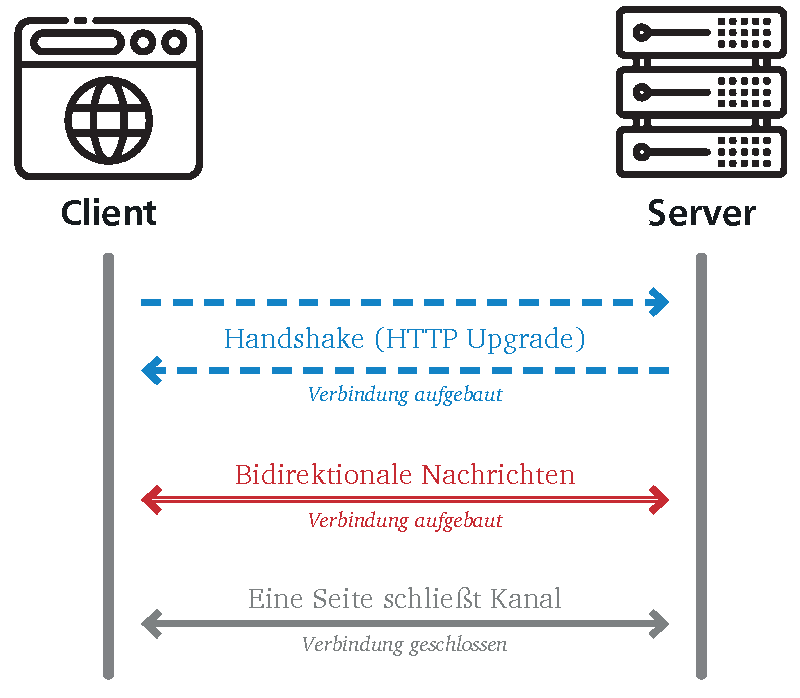
\includegraphics[width=0.7\textwidth]{images/03/WebSocket.pdf}
    \caption{Aufbau einer WebSocket Verbindung}
    \label{fig:WebSocket}
\end{figure}

WebSockets sind eine dünne Transportschicht, welche auf TCP/IP aufbaut [\cite{websockets}]. Es wird dabei allerdings nur definiert, wie der Nachrichtenaustausch stattfinden soll, nicht jedoch, wie die eigentlichen Daten innerhalb der Nachrichten strukturiert sind. Dafür werden sogenannte Unterprotokolle genutzt, welche definieren, wie die übertragenen Daten interpretiert werden sollen. Beispiele für Unterprotokolle sind JSON, XML, MQTT (Message Queuing Telemetry Transport) und WAMP (Web Application Messaging Protocol).\\
Nicht definiert wird eine Methode, mit der der Server den Client während des WebSocket-Handshakes authentifizieren kann. Dafür kann jeder clientseitiger Authentifizierungsmechanismus verwendet werden, der einem HTTP-Server zur Verfügung steht, wie etwa HTTP-Basic-Authentifizierung, JavaScript Web Tokens (JWT), oder Cookies.\\
Da WebSockets wie erwähnt direkt auf TCP/IP aufbauen statt auf HTTP, haben die Adressen für die bidirektionale Kommunikation eine Form wie \verb|ws://example.com/socket|.
